\section{Out-of-Sample Evidence and Model Risk}

{\centering
  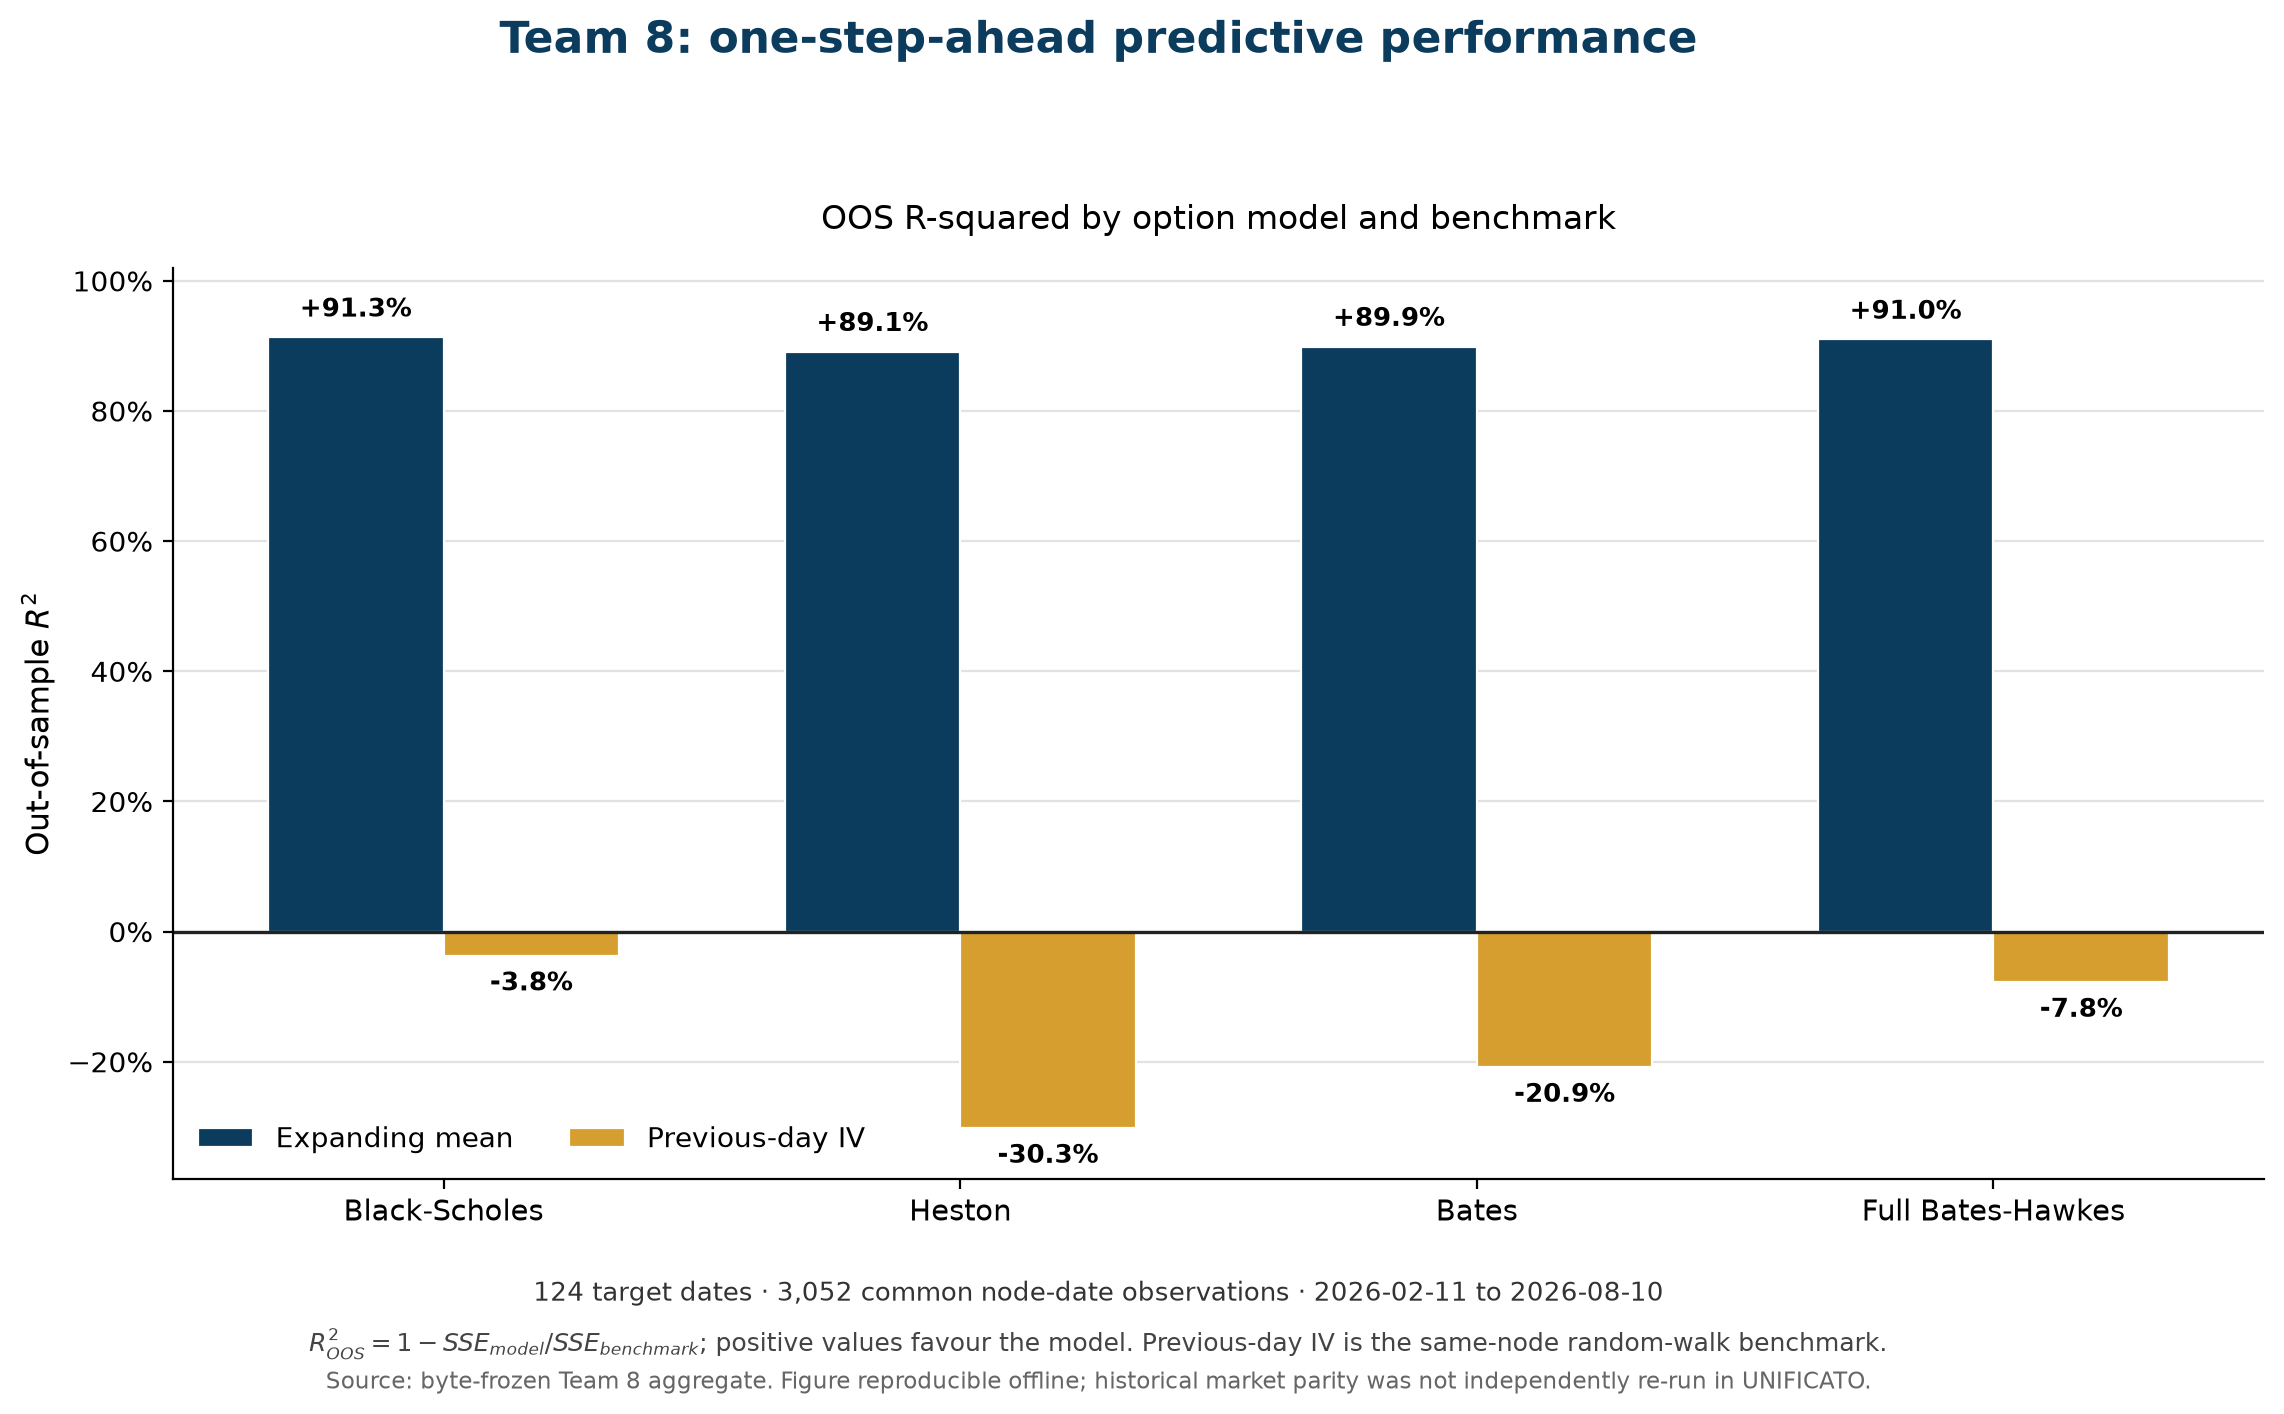
\includegraphics[width=0.95\columnwidth]{figures/online_oos_r2_by_benchmark.png}
  \captionof{figure}{One-step-ahead out-of-sample $R^2$. All four models improve on the expanding mean but fail to beat the previous-day IV surface. The test covers 124 target dates and 3,052 common node-date observations.}
  \label{fig:oos_r2}
\par}

\subsection{Predictive interpretation}
The OOS evidence prevents the in-sample ranking from being read as predictive dominance. Relative to an expanding mean, the four models explain a large share of one-step-ahead variation. Against the stronger same-node previous-day IV benchmark, every $R^2_{OOS}$ is negative; Black--Scholes also posts a slightly lower pooled RMSE than Full Bates--Hawkes. Structural flexibility therefore improves current-surface fit more clearly than short-horizon forecasting.

\begin{findingbox}[Model-risk conclusion]
Full Bates--Hawkes is primary for structural richness and current-surface calibration quality, but the valuation conclusion is reported across all four engines because the OOS evidence does not identify a dominant forecasting model.
\end{findingbox}

\subsection{Interpretive limitations}
The economic reading remains conditional: calibration is under $\mathbb Q$ without a validated $\mathbb Q\rightarrow\mathbb P$ map; GLD distributional shape is transferred without a one-for-one conversion to physical gold; market inputs are asynchronous; and the FCFF/equity bridge is not fully filing-reconciled. Debt, cash, minorities, non-operating assets and related bridge adjustments remain unresolved rather than silently inferred. The distributions are therefore research sensitivities, not fair values, confidence intervals or price targets.

{\centering
  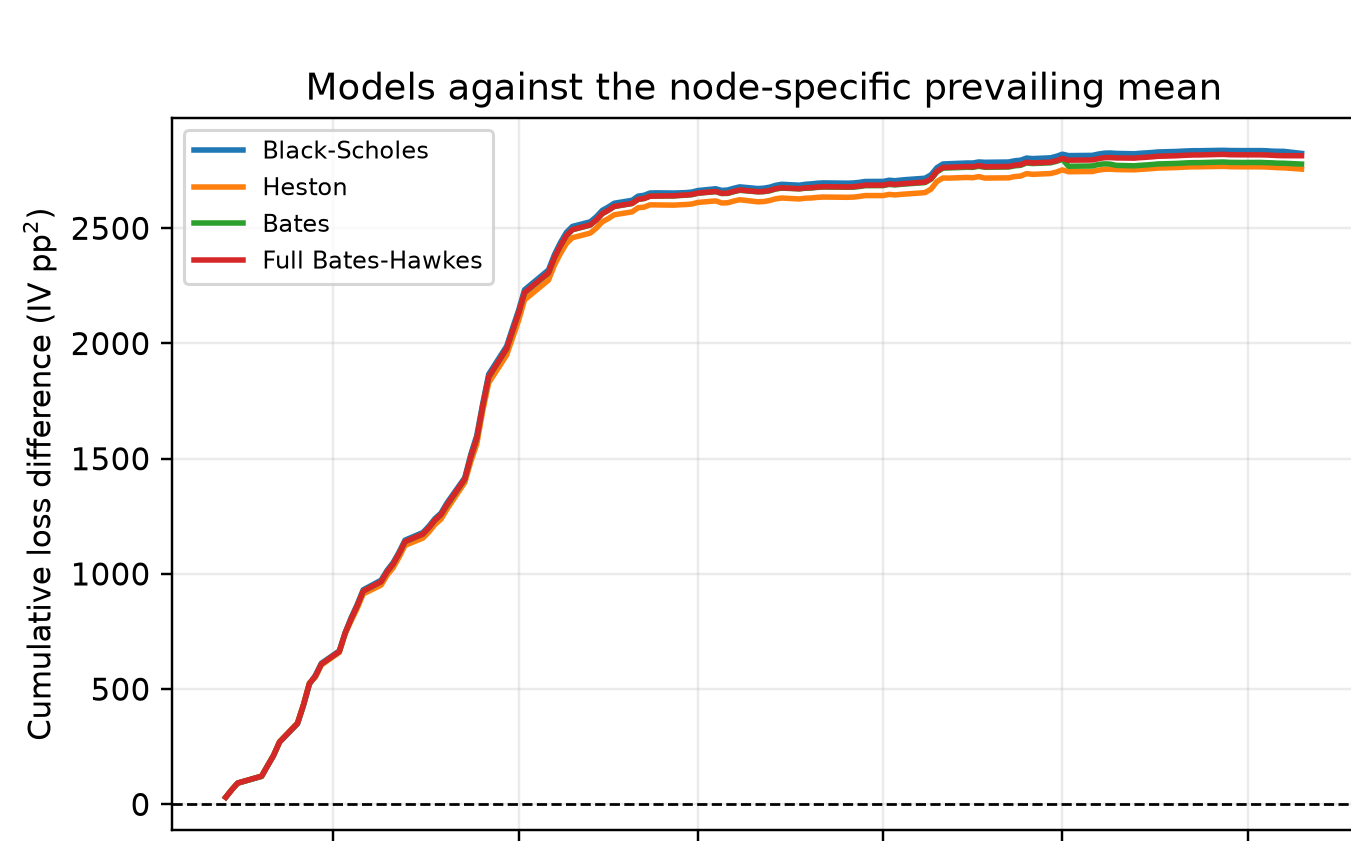
\includegraphics[width=0.95\columnwidth]{figures/welch_goyal_vs_mean.png}
  \captionof{figure}{Rolling Welch--Goyal cumulative loss difference against the node-specific prevailing mean. Upward movement favours the named model; all four specifications dominate this benchmark.}
  \label{fig:welch_goyal}
\par}


{\centering
  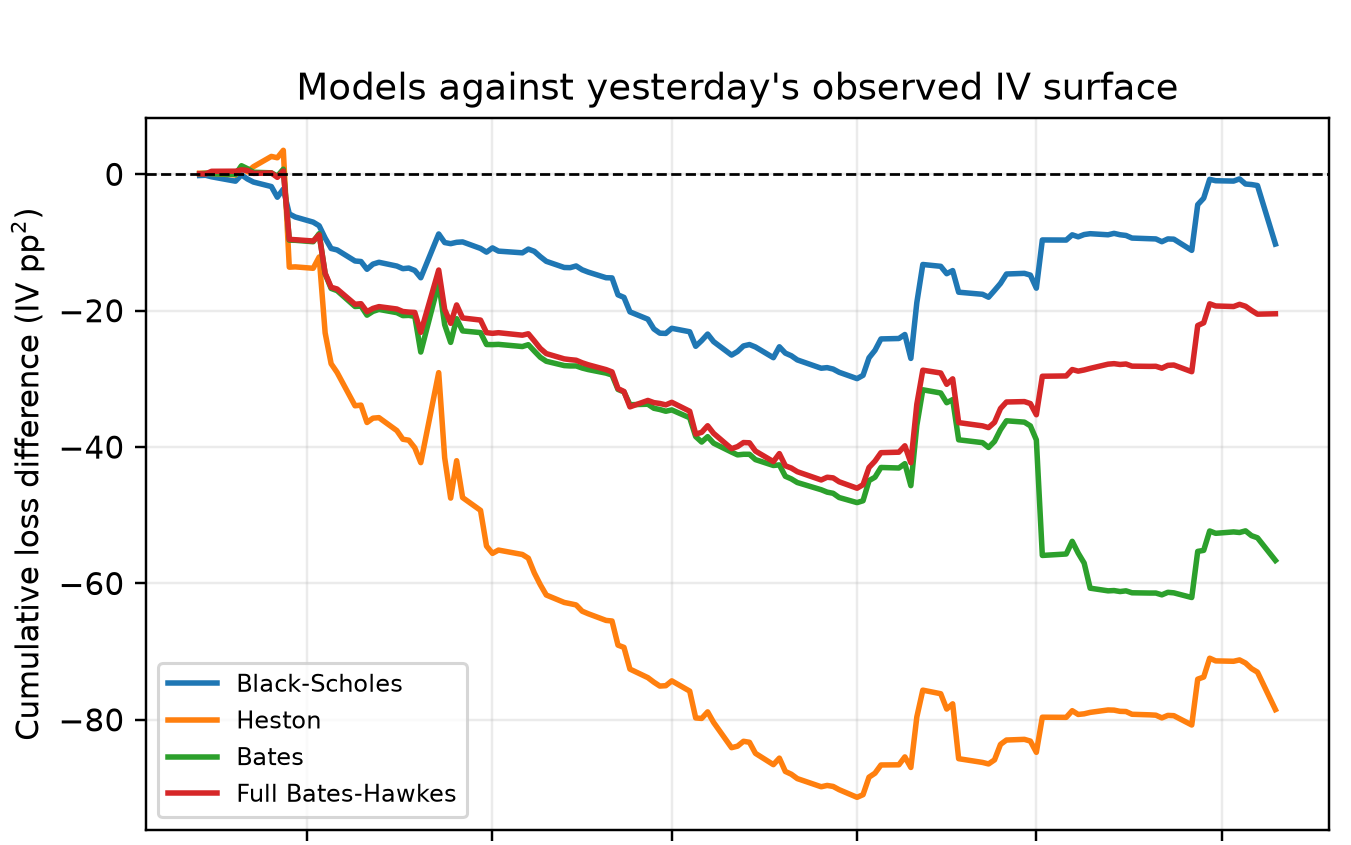
\includegraphics[width=0.95\columnwidth]{figures/welch_goyal_vs_previous_iv.png}
  \captionof*{figure}{\textbf{Figure~\ref{fig:welch_goyal} (continued).} Cumulative loss difference against the previous-day observed IV surface. Negative paths show that this stronger short-horizon benchmark remains superior.}
\par}

{\centering
  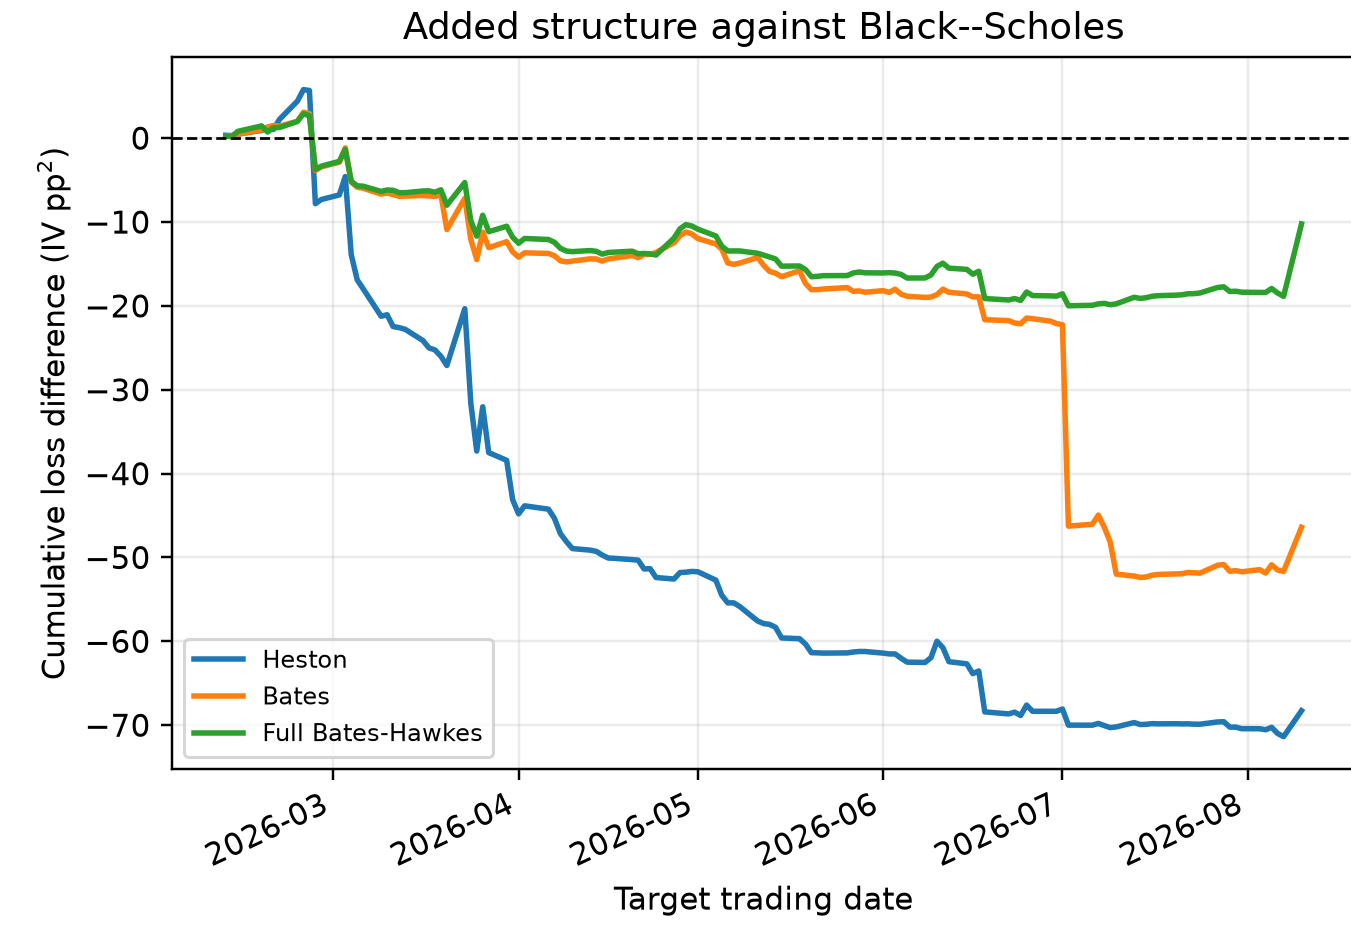
\includegraphics[width=0.95\columnwidth]{figures/welch_goyal_added_structure.png}
  \captionof*{figure}{\textbf{Figure~\ref{fig:welch_goyal} (continued).} Added stochastic-volatility and jump structure relative to Black--Scholes. Negative paths indicate that the simpler benchmark retains lower cumulative loss over this test.}
\par}

{\centering
  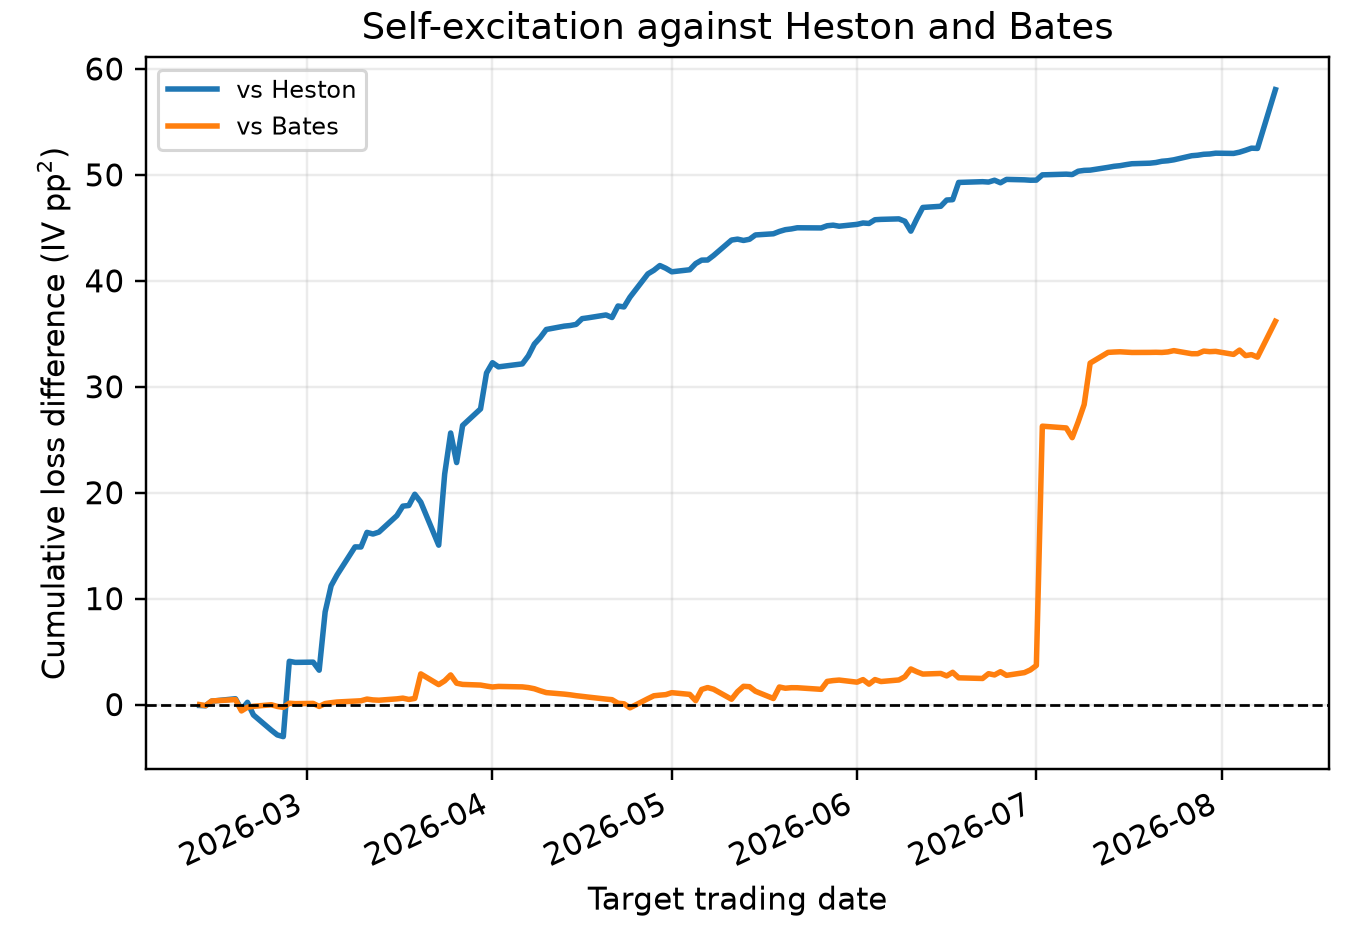
\includegraphics[width=0.95\columnwidth]{figures/welch_goyal_self_excitation.png}
  \captionof*{figure}{\textbf{Figure~\ref{fig:welch_goyal} (continued).} Full Bates--Hawkes relative to Heston and Bates. Positive paths favour the self-exciting specification within this pairwise comparison.}
\par}

\subsection{Jump-layer interpretation}
The self-exciting extension is motivated by clustered option-implied jump activity. Relative to the constant Poisson baseline, the Hawkes specification permits bursts of intensity followed by endogenous decay. In the current calibration the branching ratio is 0.02, so this channel is present but economically mild.

{\centering
  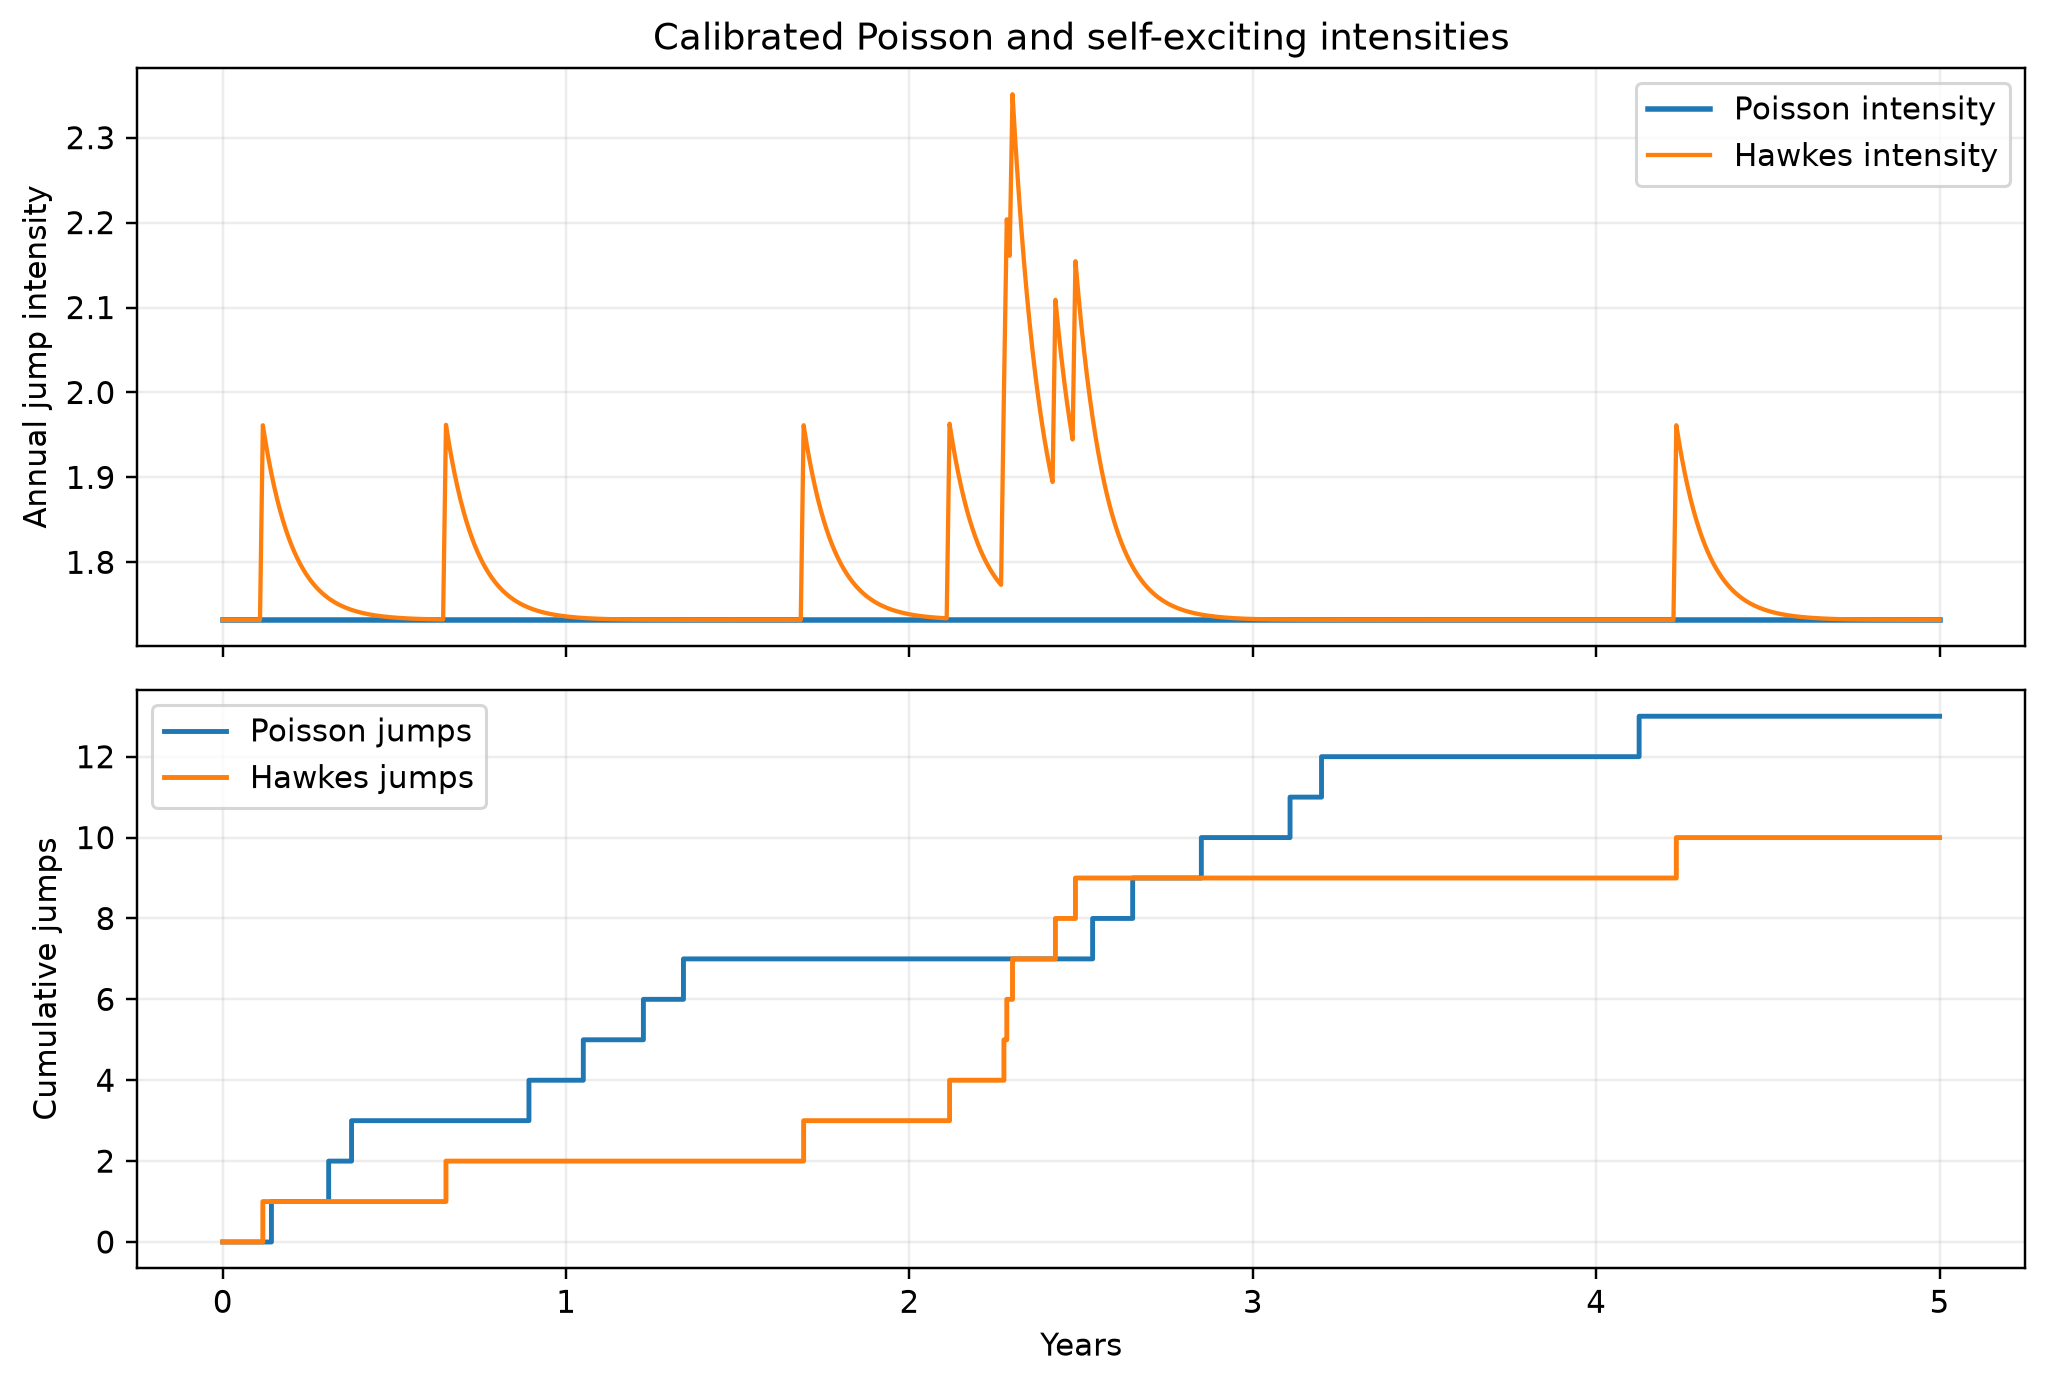
\includegraphics[width=0.95\columnwidth]{figures/hawkes_intensity_comparison.png}
  \captionof{figure}{Current Poisson and Hawkes intensity comparison. Hawkes allows clustered arrivals and decay, but the low fitted branching ratio keeps it close to the constant-intensity benchmark in this snapshot.}
  \label{fig:intensity_compare}
\par}

\section{Conclusion}

The experiment isolates the effect of stochastic gold dynamics while holding operations and corporate assumptions fixed. Under the refreshed 2 September inputs, all four conditional medians lie between USD~35.14 and USD~35.87, while the completed USD~44.13 market close remains above each median. This is a directional comparison, not a claim of market mispricing.

Model quality is multidimensional. Heston provides the strongest current-surface fit, whereas Full Bates--Hawkes produces the lowest date-equal rolling OOS loss. Its 0.5569 branching ratio is stationary but no longer economically negligible. None of the four models beats the interpolated persistence surface, although Full Bates--Hawkes comes closest. Team 4's updated operating layer uses Q1--Q2 2026 actuals and a separate Q3-onward forecast, but its uncertainty is frozen before model comparison.

The paper should therefore be read as a controlled attribution exercise. The explicit growth, WACC and terminal-value assumptions make the DCF auditable, but the terminal block still contributes about 78\% of positive enterprise value. Any fair-value interpretation would additionally require a reconciled commodity basis, physical-measure mapping, operating uncertainty and equity bridge.

\begin{findingbox}[Decision-relevant takeaway]
Under a common operating and DCF contract, changing the stochastic gold engine can affect both the central valuation signal and tail risk. The current architecture is informative for model comparison, but it is not yet a filing-reconciled fair-value model.
\end{findingbox}


\begingroup
\setlength{\bibsep}{0.6pt}
\fontsize{6.75}{7.75}\selectfont
\input{main.bbl}
\endgroup
